\documentclass{llncs}
\usepackage{amsmath}
\usepackage{amssymb}
\usepackage{bm}
\usepackage{graphicx}
\usepackage{subfigure}
\bibliographystyle{splncs}

\begin{document}

\title{Deep Networks for 3D Reconstruction from Endoscopic Video}

\author{Stephen Pizer\inst{1,2}, Julian Rosenman\inst{2,1}}
\institute{Computer Science, University of North Carolina at Chapel Hill, USA \and Radiation Oncology, University of North Carolina at Chapel Hill, USA}
\maketitle

\section{Motivation}
Endoscopy is an in-body examination procedure that enables high-resolution optical visualization of tissue texture and is a critical step in many clinical workflows. However, the use of endoscopy is still highly limited in the context of radiation therapy treatment planning due to the fact that an endoscopic video does not provide explicit 3D spatial information, thus making it difficult to use for tumor localization. In addition, due to the large amount of redundant information and lack of an efficient method to do video-based comparison, endoscopic video is almost never used for review.

Our group has proposed a pipeline in \cite{zhao16} that can reconstruct a textured 3D surface model, which we call an \textit{endoscopogram}, from multiple 2D endoscopic video frames. The model provides (1) complete 3D anatomical geometry, which facilitates tumor localization; (2) efficient visualization and comparison within and between patients; and (3) the opportunity to register endoscopy data with other modalities, such as CT, thereby enabling transfer of the tumor information into other spaces for treatment planning. We have applied this pipeline on nasopharyngoscopic and colonoscopic videos \cite{zhao16,rui16} and showed promising initial results. Preliminary clinical trials also haven shown that tumor location based on the 3D endoscopogram model can achieve within-3mm error on average.

\begin{figure}[!b]
  \centering
  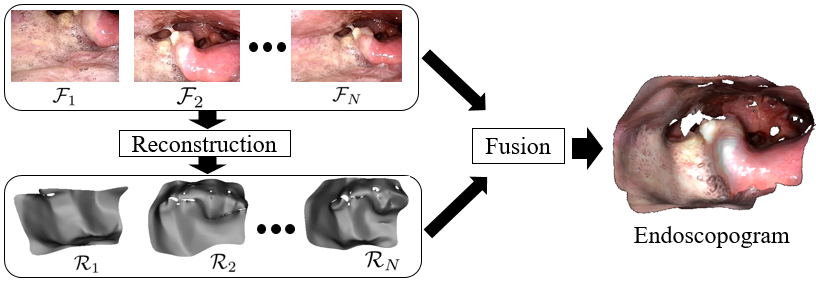
\includegraphics[height=3.5cm]{figures/pipeline}
  \caption{The endoscopogram reconstruction pipeline.}
  %\includegraphics[height=4cm]{syn.png}
  %\caption{Registration error of 24 synthetic deformations.}
\end{figure}

Our pipeline can be generally divided into two steps. First, the \textit{reconstruction} step generates for each 2D frame $\mathcal{F}_i$ a 3D reconstruction $\mathcal{R}_i$ by our novel SfMS (shape-from-Motion-and-Shading) method \cite{price16}. Then the \textit{fusion} step fuses all the single-frame reconstructions $\{\mathcal{R}_i\}$ into a single geometry $\mathcal{R}$ \cite{zhao16}. Therefore, a robust 3D reconstruction method is required in the first step, and it plays an extremely essential role in producing an accurate final result since it determines the amount of reconstruction error that is propagated into the fusion step.

\section{Existing Work and Limitations}

There have already been many attempts in applying state-of-the-art computer vision techniques in various monocular endoscopy applications \cite{armin2015,hong2014,MH2013}. In general, monocular 3D reconstruction methods can be classified into two categories: single-image-based reconstruction and multi-image-based reconstruction.

A majority of works within the scope of single-image-based reconstruction follow the line of \textit{Shape-from-Shading} (SfS) \cite{ahmed2006}. Given a single image viewing a scene, SfS can estimate the depth of the observed surface by relating the shading information with the surface normal and lighting direction. It turns out that this relationship can be formulated as a partial differential equation (PDE), which then can be solved numerically.

Multi-image based reconstruction, usually referred as Structured-from-Motion (SfM) \cite{schonberger2016}, produces a sparse scene representation from a sequence of individual frames of the endoscope video. SfM starts off by detecting and matching local image features among the set of images, then it incrementally estimates both camera poses and scene structure, which is represented by a set of 3D points.

\begin{figure}[!b]
  \centering
  % Requires \usepackage{graphicx}
  \subfigure[]{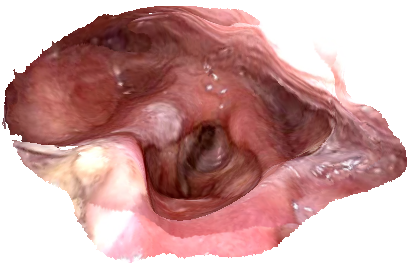
\includegraphics[height=2cm]{figures/sfms_result}}
  \subfigure[]{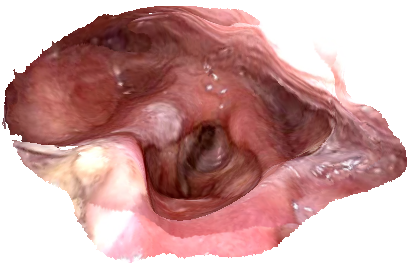
\includegraphics[height=2cm]{figures/sfms_result}}
  \subfigure[]{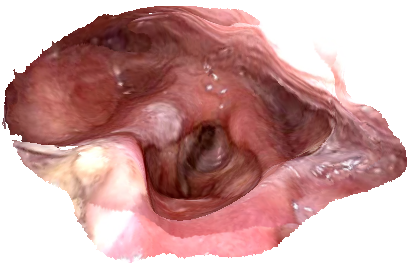
\includegraphics[height=2cm]{figures/sfms_result}}
  \caption{(a) A reconstruction result produced by our SfMS method. (b)(c) ***** You might want to put some results that can show our current limitation}
  \label{fig:sfms_result}
\end{figure}

Our group has nicely combined the two above methods into a unified Shape-from-Motion-and-Shading (SfMS) framework \cite{price16}. SfMS takes advantages from both methods, namely the sparse yet reliable 3D points detected by SfM and accurate local surface geometry estimated by SfS. It has been proven that SfMS can produce superior reconstruction results (Fig. \ref{fig:sfms_result}a). However, SfMS is still unsatisfactory to us because it suffers from the following two problems.

(1) Constant tissue deformation during endoscopy violates the scene rigidity assumption made in SfM, thus leading to polluted 3D sparse points. Non-rigid SfM methods have been proposed for some special cases, but their deformation/motion models generally don't apply for human tissues.

(2) Accurate SfS modelling relies on knowing the reflectance properties of light bouncing on tissue surfaces. This reflectance model can be highly complicated depending on tissue types. Moreover, most methods, including ours, lack the capability of modelling multiple bouncing of light in the scene, which could in turn lead to inaccurate depth estimation. Fig. \ref{fig:sfms_result}bc have shown that ****

Recent advances in computer vision focuses on applying machine learning techniques on large training datasets. In particular, with the drastically boosted parallel computing power offered by NVIDIA GPUs, it becomes possible to train deep and complex neural networks with a large amount of model parameters to fit highly nonlinear functions. Recently, deep networks also have been adopted for 3D reconstruction of natural scenes \cite{liu2015,rematas2016}. These ideas are appealing because by acquiring a large number of training data, the complicated lighting reflectance model and tissue-specific deformation model can be automatically picked up during the learning process. Hence, our next goal is to incorporate deep learning methods into our current pipeline.

\section{Deep Networks for Single Image Depth Reconstruction}

Estimating depth from a 2D image is a pixel-wise labeling problem that we need to assign a depth value to each pixel. Therefore,we follow the design of the fully convolutional neural network (FCN)[ref], which is a network used for pixel-wise segmentation, to create our deep depth estimation network. Figure 3 shows our current network design. In this network, 5 sets of convolutions and poolings are performed that downsample the image to 1/16 of its original size, then followed by two fully convolution layers to generate spacial invariant features. Afterwards, three deconvolution layers are used to upsample the output to original image size, since we are doing a per pixel-wise estimation. Finally, we use a regression type loss function to measure the difference between estimated and groundtruth depth values. Stochastic gradient descent is used to perform back propagation and update hidden parameters in the network. 

\begin{figure}[!b]
  \centering
  % Requires \usepackage{graphicx}
  \subfigure[]{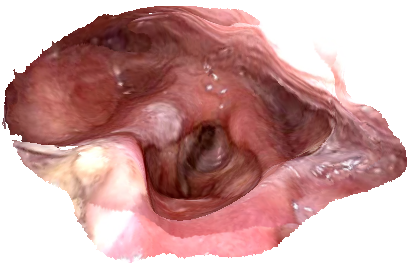
\includegraphics[height=2cm]{figures/sfms_result}}
  \subfigure[]{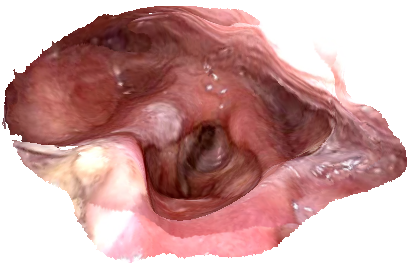
\includegraphics[height=2cm]{figures/sfms_result}}
  \subfigure[]{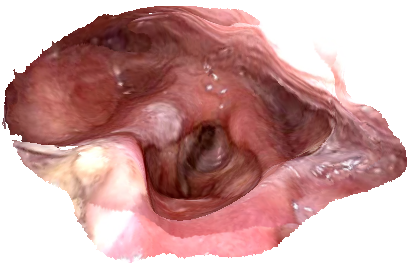
\includegraphics[height=2cm]{figures/sfms_result}}
  \caption{(a) A reconstruction result produced by our SfMS method. (b)(c) ***** You might want to put some results that can show our current limitation}
  \label{fig:sfms_result}
\end{figure}

We successfully applied our depth estimation network to 1D examples, where we create a 1D surface as our target object and generated a set of 1D intensity images by observing the 1D surface  from different angles and distances. Figure 4 illustrates our 1D synthetic data. The input to the network are intensity images and the output are their estimated depth maps. Figure 5 shows the estimated 1D depth maps together with the corresponding groundtruth depth maps.

\section{Importance of NVIDIA GPU}

Deep neural network is very powerful because of its millions of hidden parameters, which gives it the ability to model almost any complex problems. However, such network also requires a huge number of training samples. For example, the ImageNet[ref] dataset that many object classification network used for training contains millions of labeled images. However, without parallel computing power, it is almost impossible to train a deep neural network on such huge dataset. 



Even for our 1D dataset (50K 1D training images), it takes 968.83 seconds to train using CPU only, whereas it takes only 64.09 seconds to train using a NVIDIA GPU.  Therefore, it will be extremely time consuming if we train the network on 2D images using CPU. All in all, a cutting-edge NVIDIA’s GPU will be a key component to push our research work forward because its parallel computation power will allow us to train our deep depth estimation network on large medical image datasets.



\textbf{Other Related Work Published by Our Group}
See references \cite{zhao2014,zhao2015}

\textbf{Acknowledgement} This work was supported by NIH grant R01 CA158925.









\bibliography{nvidia}
\end{document}
